% =====================================================================
%  CAPÍTULO 3 — Ejemplo: resultados (tablas y figuras)
% =====================================================================
\chapter{Título del capítulo 3}\label{cap:capitulo3}

\section{Estadísticas descriptivas}

La \cref{tab:descriptivas} resume las variables principales.

% Tabla con booktabs: \toprule, \midrule, \bottomrule, sin líneas verticales.
% Si la tabla la genera Stata/R/Python, guárdela en codigo/ y use
%   \input{codigo/tabla_resultados}
\begin{table}[htbp]
  \centering
  \caption{Estadísticas descriptivas}
  \label{tab:descriptivas}
  \begin{threeparttable}
  \begin{tabular}{lrrrr}
    \toprule
    Variable & Media & Desv.\ est. & Mínimo & Máximo \\
    \midrule
    Variable 1 (\%)     & 37.92 & 14.42 & 8.40 & 65.90 \\
    Variable 2 (años)   &  9.70 &  1.13 & 7.40 & 12.70 \\
    Variable 3          &  0.77 &  0.14 & 0.53 &  0.98 \\
    \bottomrule
  \end{tabular}
  \begin{tablenotes}[flushleft]\footnotesize
    \item \textit{Fuente:} elaboración propia con datos de \ldots
  \end{tablenotes}
  \end{threeparttable}
\end{table}

\section{Resultados principales}

La \cref{fig:ejemplo} muestra \ldots

\begin{figure}[htbp]
  \centering
  % Las imágenes se buscan en figuras/ (ver \graphicspath en configuracion.tex)
  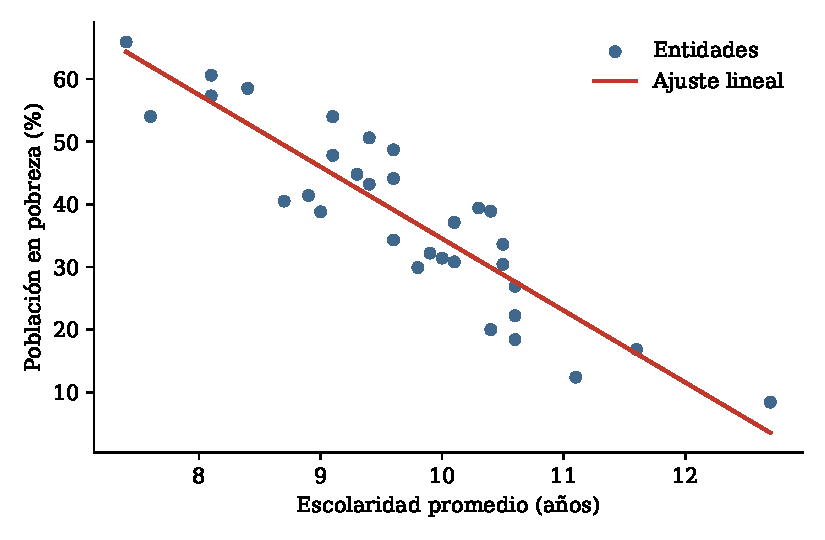
\includegraphics[width=0.75\textwidth]{figura_ejemplo}
  \caption{Título de la figura}
  \label{fig:ejemplo}
  \par\footnotesize\textit{Fuente:} elaboración propia.
\end{figure}

\lipsum[11-12]
